\chapter{Evaluation of NMR data for examining IL-10-GAG interaction}

The combination of both, \textit{in silico} methods and nuclear magnetic
resonance (NMR) data, often leads to an improved understanding of the system
under investigation, compared to the insights obtained with either approach
individually. This is especially true for protein-GAG systems, where \textit{in
silico} simulations are usually performed based on NMR data in order to obtain a
structural model with larger spatial resolution than achievable from NMR data
alone. The principal complementarity of NMR and \textit{in silico} methods with
respect to protein-GAG systems is broad and has been demonstrated and published
before, for instance in \cite{pichert_characterization_2012, sost_heparin_2009,
nieto_conf_selection_heparin_2011}.

In an ongoing effort, G. Künze from Prof. D. Huster's laboratory at the
Universität Leipzig investigates the IL-10-GAG system with NMR methods. In this
chapter, I describe how I post-processed his nuclear Overhauser effect
spectroscopy data in order to derive heparin tetrasaccharide structure models
for the free state (without IL-10 in solution) and bound state (with IL-10 in
solution) and discuss the implications of the corresponding results. This work
is part of our collaborative publication titled \enquote{NMR characterization of
the binding properties and conformation of glycosaminoglycans interacting with
interleukin-10} in the \textit{Glycobiology} journal \cite{kuenze_gehrcke_2014}.
Additionally, in this chapter I summarize further insights derived from G.
Künze's data and discuss them in the context of the conclusions drawn in this
thesis so far.

%The combination of insights gained via \textit{in silico} methods and
%experimentally obtained data has led to an improved understanding of the
%molecular recognition principles governing the IL-10-GAG system. This chapter
%presents the studies and outcomes of this collaborative effort.

\section{Heparin structure calculation for the bound and unbound state}

\subsection{Background: NOESY for inter-atomic distance determination}
\label{nmr:noesy_background}

In essence, the spins of atomic nuclei that are spatially close to each other
(closer than about \SI{5}{\angstrom}) may undergo a significant dipole-dipole
interaction, leading to the measurable effect of nuclear spin polarization
transfer from one nuclear spin population to another. In other words, after
excitation, two dipolar-coupled spins do not relax independently, which is
called the nuclear Overhauser effect (NOE). In two-dimensional nuclear
Overhauser effect spectroscopy (NOESY) experiments, this correlation effect
manifests itself in form of off-diagonal resonance peaks. In first order
approximation (or \enquote{isolated two-spin approximation}), the intensity of
such a so-called cross peak is proportional to the cross-relaxation rate
constant for the two-spin system. Due to the dipolar nature of this spin-spin
interaction, the rate constant is proportional to the inverse sixth power of
the distance between the two spins \cite{neuhaus2000_noe}. Likewise, the main
usage of the nuclear Overhauser effect in NMR spectroscopy for biological
questions is the detection of distances between pairs of protons. Eventually and
under ideal conditions, NOESY can be used for collecting sufficient geometrical
information about a certain molecule for determining a three-dimensional
structure of that molecule (obviously, this requires knowledge about the
chemical configuration of that molecule as well as a mapping between cross peaks
and atom pairs). In practice, depending on the environmental conditions and on
the type of molecule investigated, there are various sources of error that can
prevent NOE cross peaks from building up, or that significantly invalidate the
assumption of a linear dependence between the peak intensity and the relaxation
rate constant \cite{palmer_online_nmr_relaxation}, affecting at least the
spatial resolution of the data, or even the ability to obtain meaningful NOE
data at all.


\subsection{Methods} \label{nmr:methdos} G. Künze carried out nuclear Overhauser
effect spectroscopy experiments for measuring GAG-internal hydrogen-hydrogen
(${}^1$H-${}^1$H) NOE cross peaks of heparin tetrasaccharide (HP dp4) molecules
in solution, in two different conditions: under presence of murine IL-10 in the
very same solution, and without presence of IL-10. The protocol details of these
experiments have been published in \cite{kuenze_gehrcke_2014}. The aim of these
experiments was to extract and use the geometry information encoded in the
resulting NOESY data, for creating two HP dp4 structure models: one for what we
call the \enquote{bound} state, and one for the \enquote{unbound} state (with
and without IL-10, respectively).

The creation of structure models from the NOESY-derived distance data can be
considered an optimization problem --- with the goal of finding the heparin
structure fulfilling the experimentally obtained cartesian distance constraints
as good as possible. I have approached this optimization problem with simulated
annealing molecular dynamics simulations, a classical minimization method
applicable in this scenario \cite{nilges_sim_annealing_noe_1988}.

HP dp4-internal ${}^1$H-${}^1$H distances were calculated from experimentally
obtained NOE intensities assuming a $1/r^6$ distance dependence between
interacting protons, as justified in \cref{nmr:noesy_background}. The
calibration was based on the H2-H4 and H3-H5 proton pairs of the GlcNS,6S ring
(atom nomenclature according to IUPAC rules) with a known distance of
\SI{2.55}{\angstrom} in the ${}^4$C${}_1$ chair conformation. A tolerance
interval of $\pm \SI{0.3}{\angstrom}$, $\pm \SI{0.6}{\angstrom}$ and $\pm
\SI{1.0}{\angstrom}$ was specified for measured distances $<
\SI{2.0}{\angstrom}$, between \num{2.0} and $\SI{4.0}{\angstrom}$, and $>
\SI{4.0}{\angstrom}$, respectively. The corresponding raw distance data is
enlisted in the supplementary material of \cite{kuenze_gehrcke_2014}.

The experimentally obtained distance restraints were subsequently used for GAG
structure determination using MD simulated annealing simulations employing the
NMR distance restraint functionality implemented in the PMEMD module of Amber 12
\cite{case_amber_12}. Atom types of the GLYCAM 06g force field
\cite{kirschner_glycam06:_2008} were used to build the heparin tetrasaccharide
IdoA,2S-GlcNS,6S-IdoA,2S-GlcNS,6S, referred to as rings A, B, C, D,
respectively. Sulfate partial charges, which are not provided within GLYCAM,
were obtained from RESP calculations for methylsulfate at the 6-31(d)G level of
theory --- in consistence with the other parts of the force field. The heparin
molecules used in the NMR experiments were prepared by enzymatic digestion, so
the non-reducing terminal uronic acid became unsaturated. Since GLYCAM does not
contain proper parameters for 4,5-unsaturated uronic acid, the non-reducing
terminal acid was modeled as IdoA,2S and NOE signals involving hydrogens of ring
A other than H1 were not applied as restraints in the simulations. Generally,
the structure generation was performed in a custom two-step protocol, first by
structure optimization in \textit{implicit} solvent, and subsequent refinement
in \textit{explicit} solvent. The two stages were repeated many times, yielding
an ensemble of structure models. In various test runs, the simulate annealing
protocol details were iteratively adjusted and improved in order to obtain
convergence in the solution to the optimization problem.

The first structure optimization stage was a simulated annealing protocol using
a simple implicit solvent model with a $1/r$ distance dependency of the
dielectric constant. The goal of this stage was to quickly guide the heparin
conformation by the distance restraints, without introducing degrees of freedom
for explicit water molecules, which would generate noise and impede the
convergence of the minimization process. The protocol contained the following
steps: \textit{i)} steepest descent and conjugate gradient minimization without
restraints, \textit{ii)} 100 ps MD with tight coupling to a \SI{600}{\kelvin}
heat bath and gradual activation of NMR distance restraints, \textit{iii)}
\SI{300}{\pico\second} MD with restraints, gradual temperature change from
\SI{600}{\kelvin} to \SI{10}{\kelvin}, and normal coupling to heat bath,
\textit{iv)} short MD with gradual cooling to \SI{0}{\kelvin} and tight coupling
to heat bath. The MD time step for this protocol was set to
\SI{1}{\femto\second}. The second optimization stage was performed with periodic
boundary conditions in TIP3P explicit solvent (with at least \SI{8}{\angstrom}
from all solute atoms to the box boundary), with Na+ ions for system
neutralization, using SHAKE, and with an MD time step of \SI{2}{\femto\second}.
The goal of this stage was to incorporate the electrostatic repulsion among the
charged groups in the heparin molecule as realistic as possible using classical
molecular mechanics force fields. The following steps were performed:
\textit{i)} solvent minimization with constrained solute, \textit{ii)}
\SI{20}{\pico\second} heat up MD to \SI{300}{\kelvin} in NVT ensemble with
strong positional restraints on solute atoms, \textit{iii)}
\SI{200}{\pico\second} equilibration MD in NPT with weak positional restraints
on solute atoms and NMR distance restraints, \textit{iv)}
\SI{200}{\pico\second} MD in NPT with NMR distance restraints and a gradual
cooling to \SI{250}{\kelvin}, \textit{v)} \SI{400}{\pico\second} MD in NPT with
NMR distance restraints and a gradual cooling to \SI{0}{\kelvin}. Beyond the
tolerance interval, each NMR distance restraint was implemented with a harmonic
potential with a force constant of
\SI{20}{\kilo\calory\per\mole\per\angstrom\squared}. The two stages of structure
optimization were repeated 100 times in independent simulations with different
random seeds. All optimized structures were aligned to each other. Structure
alignment was based on all ring atoms of rings B, C, D, and all glycosidic
linkage oxygens. The root mean square distance (RMSD) among these atoms was
calculated to obtain the structural distance between any two given structures.
The \textit{structural diversity} within the ensemble was quantified by
calculating the mean pairwise structural distance among all aligned structures.
The structure having the lowest mean structural distance to all other structures
in the ensemble was selected as the representative of the ensemble.

For structure characterization, the distribution of various dihedral angles was
evaluated for all structures in an ensemble. For analyzing the GAG backbone
structure, we measured the glycosidic linkage torsional angles Φ, defined by
atoms H1-C1-O4-C4, and Ψ, defined by C1-O4-C4-H4, both in direction from the
non-reducing end to the reducing end of the GAG. Additionally, the orientation
of sulfate side-chains was measured via the dihedral angles H2-C2-O-S for
2-O-sulfates, H2-C2-N-H for 2-N-sulfates, and O5-C5-C6-O6 for 6-O-sulfates.

\subsection{Results and discussion}
\label{nmr:results_discussion}

\begin{figure}
\centering
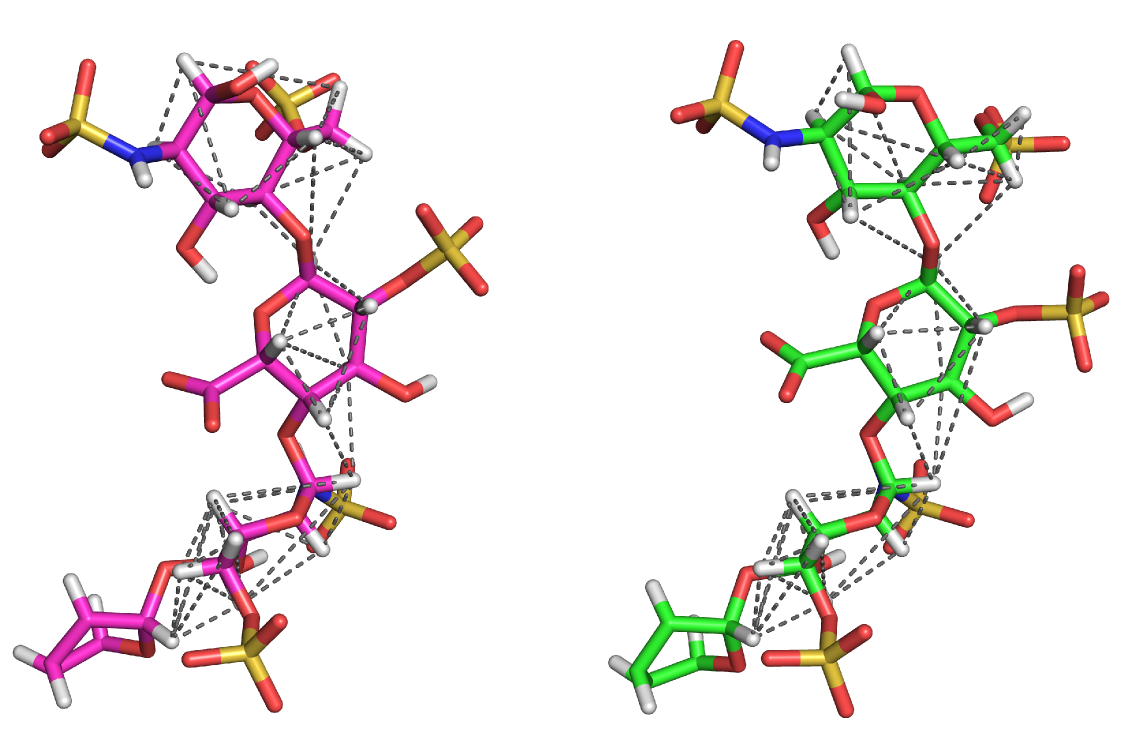
\includegraphics[width=0.7\textwidth]{gfx/nmr/two_cases_dashed_lines_distances.png}
\caption[]{
Heparin tetrasaccharide-internal H-H distance restraints applied during
simulated annealing MD simulations. Each dashed line corresponds to one NMR
distance restraint. In the unbound case (left, carbon in magenta), 42
restraints were applied. In the bound case (right, carbon in green), 41
restraints were used. Functional groups of ring A are not shown for clarity.
Atoms are color-coded with red, blue, yellow, gray corresponding to oxygen,
nitrogen, sulfur, and hydrogen, respectively.
}
\label{fig:nmr:hp_dashed_lines_distances}
\end{figure}

\begin{figure}
\centering
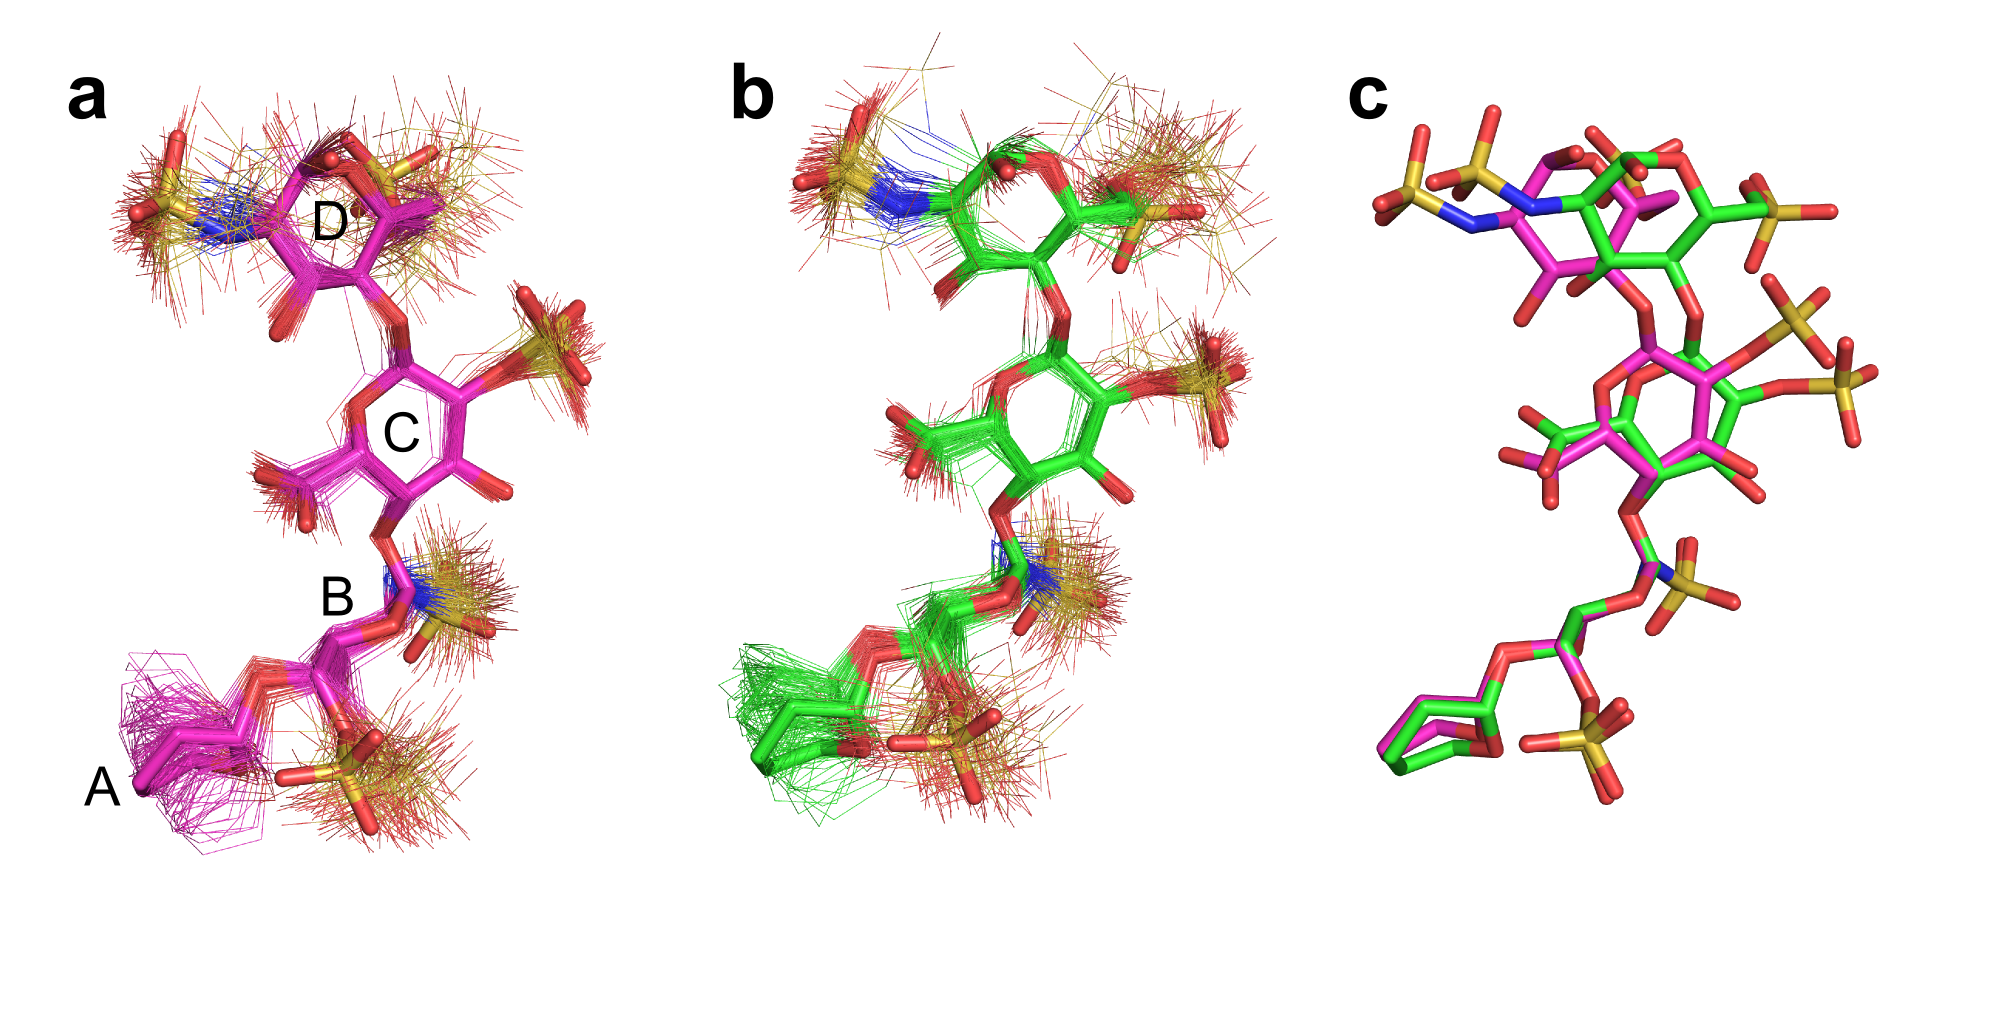
\includegraphics[width=\textwidth]{gfx/nmr/Figure_07_bound_vs_free_three_panels_05.png}
\caption[]{
Heparin structure models obtained from NOE data and simulated annealing
simulations. (a) structure model ensemble for the unbound case (ring identifiers
in capital letters). (b) structure model ensemble for the bound case. (c) the
representative structure for both, the unbound (carbons in magenta) and bound
(carbons in green) ensembles, aligned on ring B. The ensemble representatives
are shown in thick sticks. Functional groups of ring A and hydrogens are not
shown for clarity. Atoms are colored by type (oxygen: red, nitrogen: blue,
sulfur: yellow).
}
\label{fig:nmr:hp_ensembles_representatives}
\end{figure}


% Two tables side by side, same caption
% from http://tex.stackexchange.com/a/2836
\begin{table}
\footnotesize
%\centering
\renewcommand{\arraystretch}{1.3}
\begin{tabular}{llc}
\multicolumn{3}{c}{Unbound case} \\
\midrule
proton 1  & proton 2 & violation (\si{\angstrom}) \\
\midrule
B H5 & B H62 & 0.000 $\pm$ 0.001 \\
B H5 & B H61 & 0.000 $\pm$ 0.001 \\
C H1 & D H4 & 0.000 $\pm$ 0.002 \\
A H1 & B H4 & 0.000 $\pm$ 0.002 \\
D H5 & D H3 & 0.001 $\pm$ 0.007 \\
C H2 & C H5 & 0.003 $\pm$ 0.012 \\
B H3 & B H5 & 0.005 $\pm$ 0.014 \\
D H2 & D H4 & 0.006 $\pm$ 0.028 \\
A H1 & B H62 & 0.010 $\pm$ 0.021 \\
B H2 & B H4 & 0.017 $\pm$ 0.027 \\
B H1 & C H3 & 0.019 $\pm$ 0.031 \\
C H1 & D H62 & 0.026 $\pm$ 0.038 \\
B H1 & C H4 & 0.037 $\pm$ 0.045 \\
B H62 & B H4 & 0.037 $\pm$ 0.045 \\
A H1 & B H61 & 0.040 $\pm$ 0.053 \\
C H4 & C H2 & 0.052 $\pm$ 0.041 \\
D H62 & D H4 & 0.053 $\pm$ 0.050 \\
C H1 & C H2 & 0.059 $\pm$ 0.020 \\
D H5 & D H61 & 0.074 $\pm$ 0.026 \\
C H3 & C H5 & 0.084 $\pm$ 0.017 \\
C H4 & C H3 & 0.102 $\pm$ 0.014 \\
D H1 & D H61 & 0.150 $\pm$ 0.061 \\
D H5 & D H62 & 0.161 $\pm$ 0.023 \\
A H1 & B H3 & 0.236 $\pm$ 0.057 \\
\midrule
\end{tabular}
\quad
\begin{tabular}{llc}
\multicolumn{3}{c}{Bound case} \\
\midrule
proton 1  & proton 2 & violation (\si{\angstrom}) \\
\midrule
B H1 & C H4 & 0.000 $\pm$ 0.001 \\
B H62 & B H4 & 0.000 $\pm$ 0.001 \\
A H1 & B H4 & 0.000 $\pm$ 0.001 \\
B H5 & B H62 & 0.001 $\pm$ 0.006 \\
D H2 & D H4 & 0.001 $\pm$ 0.008 \\
C H1 & D H4 & 0.005 $\pm$ 0.049 \\
A H1 & B H61 & 0.009 $\pm$ 0.019 \\
A H1 & B H62 & 0.010 $\pm$ 0.021 \\
D H1 & D H4 & 0.015 $\pm$ 0.028 \\
B H1 & C H3 & 0.018 $\pm$ 0.036 \\
C H2 & C H5 & 0.023 $\pm$ 0.083 \\
C H1 & D H62 & 0.053 $\pm$ 0.041 \\
A H1 & B H3 & 0.121 $\pm$ 0.024 \\
B H1 & C H2 & 0.176 $\pm$ 0.049 \\
C H1 & D H3 & 0.195 $\pm$ 0.059 \\
\midrule
\end{tabular}
\caption{
Cartesian distance restraint violations in the final ensemble of optimized
structures for the unbound (left) and bound (right) case. The violation, i.e.\
the deviation from the NOE-derived proton-proton distance tolerance interval, is
given with its mean value $\pm$ standard deviation (built from the entire
ensemble with 100 structures). Violations with a mean value and standard
deviation smaller than \SI{0.000}{\angstrom} are not listed. H61 is H6-proS and
H62 is H6-proR, according to the considerations made in
\cite{nishida_rotameric_nmr_1988}. The other hydrogens are named in compliance
to IUPAC nomenclature.}
\label{tab:nmr:restraint_viols_free}
\end{table}


Structural models of HP dp4 were created by performing simulated annealing MD
simulations including NOE-based hydrogen pair distance restraints, for the
unbound HP dp4 and for HP dp4 in the presence of IL-10. In the unbound case, 42
H-H distance restraints were applied during the simulations (visualized in
\cref{fig:nmr:hp_dashed_lines_distances}). In the ensemble of optimized
structures, about half of the restrained hydrogen pairs show a minor deviation
from their corresponding distance restraint tolerance interval, as listed in
\cref{tab:nmr:restraint_viols_free}. That is, the geometrical data obtained via
NMR measurements is largely in compliance with the potentials defined by the
GLYCAM force field. The ensemble has a structural diversity (defined in
\cref{nmr:methdos}) of \SI{0.37}{\angstrom}
(see \cref{fig:nmr:hp_ensembles_representatives}a), i.e.\ it is well-converged,
meaning that the applied simulated annealing optimization procedure was
sufficiently tuned for the kind of data used in this study. In the bound state,
the distance of 41 hydrogen pairs was restrained, as visualized in
\cref{fig:nmr:hp_dashed_lines_distances}. About a fourth of them show a minor
deviation from the tolerance interval, as listed in
\cref{tab:nmr:restraint_viols_free}. The resulting ensemble is also
well-converged, with a structural diversity of \SI{0.43}{\angstrom}, as
visualized in \cref{fig:nmr:hp_ensembles_representatives}b.

During the MD simulations, the NOE distance restraints involving hydrogens of
ring A other than H1 were not applied (as of the inaccurate parameterization of
the GLYCAM force field for the 4,5-unsaturated acid ring). Since the unsaturated
uronic acid ring plays no functional role for the biology of heparin, the
structural details of this ring are not discussed here --- an approach which has
also been taken by Jin et al. \cite{jin_heparin_2009}. Hence, functional groups
of ring A are not shown in \cref{fig:nmr:hp_ensembles_representatives}.

Overall, the NOE distance data and MD simulations have led to valid heparin
structure models. In both, the bound and unbound case, the ensemble
representatives have their rings in valid conformations, namely ring B in
${}^4$C${}_1$, ring C in ${}^2$S${}_\mathrm{O}$, and ring D in ${}^4$C${}_1$
conformation. Also the distribution of glycosidic linkage torsional angles is in
a valid range of values, as observed in free heparin microsecond MD simulations
and in bound and unbound heparin structures found in the PDB. The overall
conformation observed in the heparin structure models is consistent with one of
the earliest heparin structure models previously obtained via NMR and modeling
\cite{foster_mulloy_1993}.

\begin{figure}
\begin{adjustwidth}{-1cm}{-1cm}
\centering
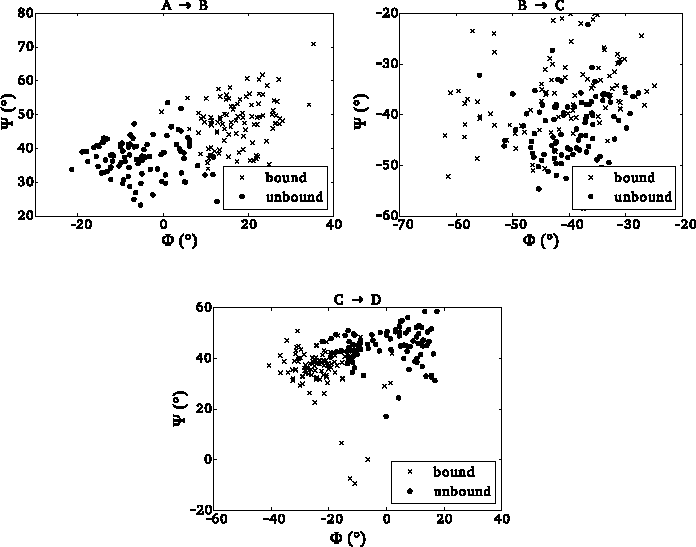
\includegraphics[width=1.1\textwidth]{gfx/nmr/glycolinkage_dihedrals_bound_vs_free_3panels_03.pdf}
\caption[]{
Glycosidic linkage torsional angle distributions of heparin structure model
ensembles obtained from simulated annealing simulations involving NMR distance
restraints. Data comparing the bound and unbound state is shown individually for
each linkage in the heparin tetrasaccharide, namely for linkages A
\rightarrow B, B \rightarrow C, and C \rightarrow D.
}
\label{fig:nmr:hp_glyco_dihedral_distributions}
\end{adjustwidth}
\end{figure}

One of the major observations to be made from the two heparin structure
ensembles is that there is a slight difference in the overall GAG backbone
structure between the bound and unbound cases, as can be inferred from the
structure alignment shown in \cref{fig:nmr:hp_ensembles_representatives}c. The
generated structure models let us conclude that the bound heparin is less bent
than its free form. This small but significant difference was further quantified
by evaluating the distribution of glycosidic linkage torsional angles in both
structure ensembles, see \cref{fig:nmr:hp_glyco_dihedral_distributions}. A
significant change in the Φ distribution of linkage A→B, a shift in the Ψ
distribution of linkage B→C, and a significant shift in the Φ distribution of
linkage C→D can be observed. Although the reliability of single certain distance
restraints derived from NOE data may surely be questioned, the pure existence of
a difference in shown glycosidic linkage torsional angle distributions must be
considered meaningful, since the raw NOE data for the two cases was obtained in
a highly consistent and reproducible manner. It should be noted that the
seemingly small backbone structure difference between the bound and unbound
cases should not be interpreted in terms of IL-10-GAG interaction affinity: even
in the high affinity complex comprised of bFGF and a heparin tetrasaccharide
\cite{faham_heparin_1996,mikhailov_hp_tetra_1996} the backbone differences
between bound and unbound GAG are rather small. The conclusion to be made from
these data is that IL-10-HP interaction has a measurable impact on the HP
structure.

\begin{figure}
\centering
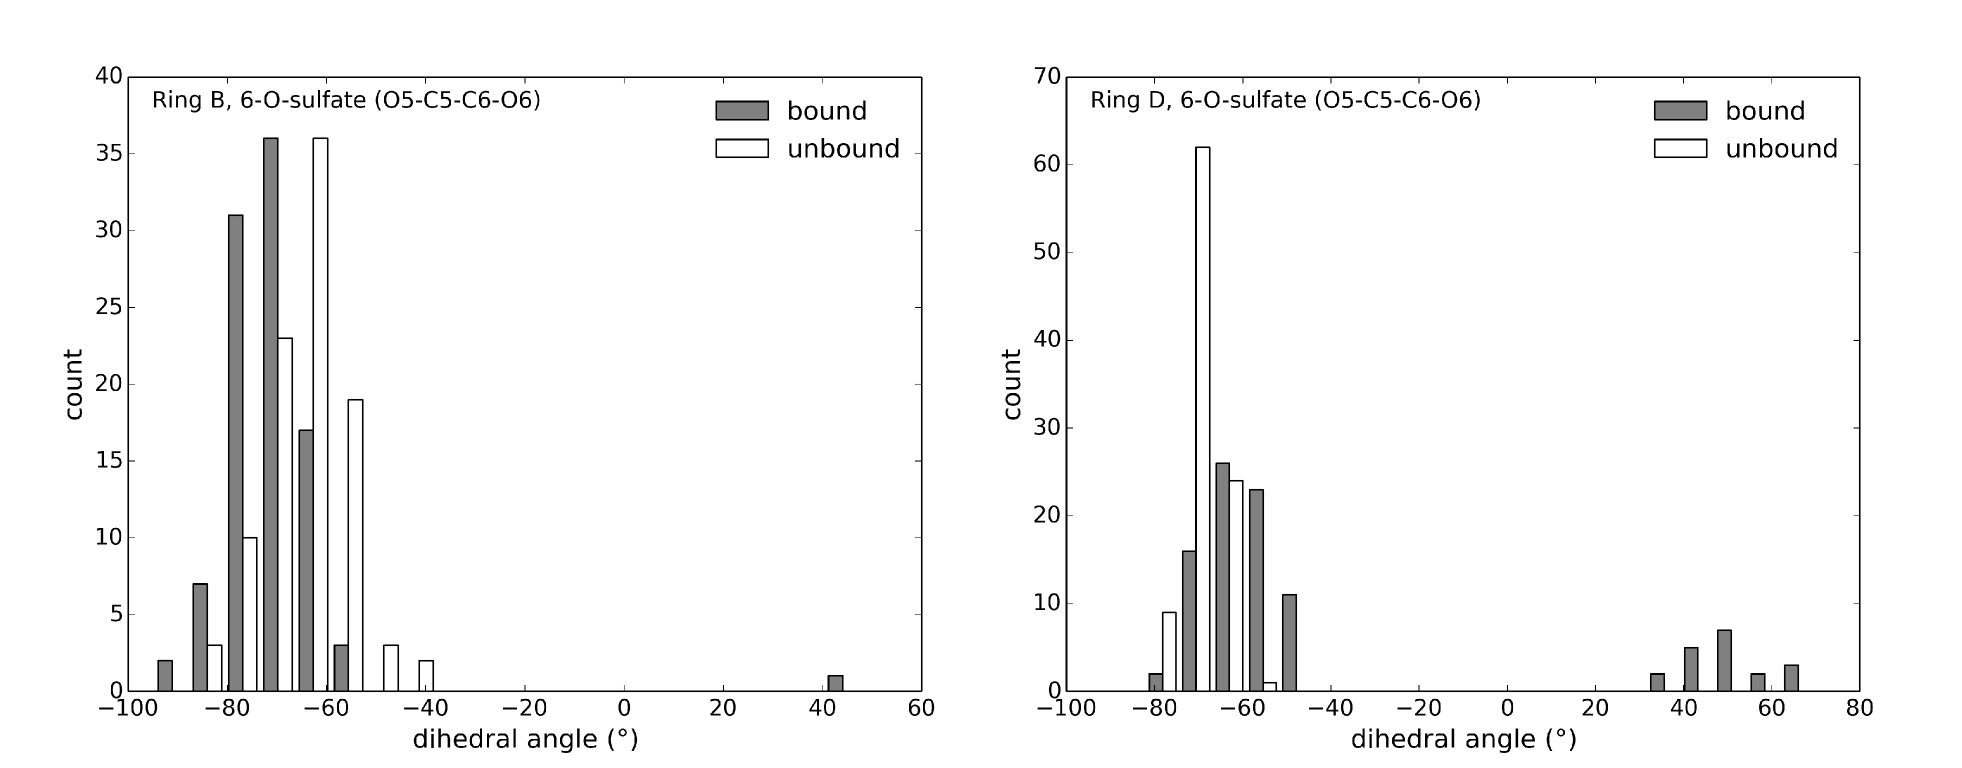
\includegraphics[width=\textwidth]{gfx/nmr/SI_figure_6O_sulfate_dihedrals_B_D_01.png}
\caption[]{
Distribution of 6-O-sulfate orientations in heparin tetrasaccharide structure
models obtained from obtained from simulated annealing simulations involving NMR
distance restraints, in comparison for the bound and unbound state.}
\label{fig:nmr:hp_sulfate_orientations}
\end{figure}


Apart from the glycosidic linkage angular distributions, also the orientation of
the sulfate groups in the structure ensembles was investigated via the
evaluation of dihedral angles. In case of four of the six sulfate groups, the
orientation does not differ significantly between the bound and unbound state.
That is, according to our heparin structure ensembles, the orientation of most
functional groups of rings B, C, and D is conserved among the bound and unbound
ensembles. Notable exceptions are the 6-O-sulfate groups of ring B and D, which
were observed to be affected by the presence of IL-10 (see
\cref{fig:nmr:hp_sulfate_orientations}). In ring B, the 6-O-sulfate has
converged purely towards the \textit{gauche-gauche} rotamer state in both cases,
but there is a slight shift between the rotamer distributions of the unbound and
bound state: in the bound state the 6-O-sulfate of ring B deviates by about
\SI{10}{\degree} from the ideal rotation angle of \SI{-60}{\degree}.
For the 6-O-sulfate of ring D there is a larger difference between the two
cases. It only populated the \textit{gauche-gauche} rotamer state in the unbound
case, and showed a significant additional population of the
\textit{gauche-trans} conformer (\SI{60}{\degree}) in the bound case. The
meaning of these observations is further discussed in
\cref{nmr:further_insights}, together with the corresponding direct NMR
measurements.

%
%\SI{-10}{\degree} of the rotamer distribution in the bound heparin structure. In
%ring C an additional fraction of the \textit {gauche-trans} conformer in the
%presence of IL-10 is observed.

%3J couplings between H5 and H6 protons%
% Further information on the conformation of 6-O-sulfate side
%chains was revealed from , \hl{as
%discussed in} .

It is important to stress again that the entire structure modeling approach as
described above is based on the isolated two-spin approximation (in which the
intensity of single NOE cross peaks is assumed to be linearly dependent on the
inverse sixth power of the proton-proton distance) and therefore is
intrinsically error-prone to an unknown extent. A realistic estimation of the
corresponding error of the final Cartesian coordinates of the obtained structure
models would require more sophisticated NMR measurements and full relaxation
matrix calculations, as performed in the more thorough works of Mulloy et al.
\cite{foster_mulloy_1993} and Mikhailov et al. \cite{mikhailov_hp_tetra_1996}.
While the structures obtained here can be considered valid to a certain degree
\cite{jones_noe_2011}, they should not in all detail be taken literally. The
observed differences between the bound and unbound case, however, are of
significance, since all systematic errors introduced in the work flow are the
same in both cases.

%\hl{Note (TODO):}
%\hl{Discuss what this HEPARIN STRUCTURE now brings us for clarifying atomic
%detail interaction.. speculate: DMD with inflexible GAG ligand?}

\section{Further insights revealed by NMR experiments}
\label{nmr:further_insights}

An important point also published in our collaborative work
\cite{kuenze_gehrcke_2014} is the direct observation of the rotamer state
distribution of the 6-O-sulfate groups via ${}^{3}$J coupling measurements
between the protons H5 and H6 of the monosaccharides comprising the heparin
molecule --- in the unbound state. Using the Karplus approach
\cite{haasnoot_karplus_1980,nishida_rotameric_nmr_1988}, the C5-C6 bond of both
GlcNS,6S rings (B and D) was determined to be in \textit{gauche-gauche} state
with a probability of \SI{70}{\percent}, and in  \textit{gauche-trans} state
with a probability of \SI{30}{\percent}. This is in compliance to the ratio
observed for other glucopyranoses \cite{nishida_rotameric_nmr_1988}.
Unfortunately, a precise comparative measurement of the H5-H6 couplings for the
bound case (with IL-10 in solution) was prevented by peak broadening. Hence, no
direct comparison between the bound and unbound cases was possible. In the
previous section, the heparin structure ensemble of the unbound case was found
to have the 6-O-sulfates only in \textit{gauche-gauche} orientation. This is
contradicting the direct NMR measurement just described and suggests that the
sulfate rotamer distribution as yielded by the MD structure optimization
protocol is over-sensitive to small variations in single distance restraints and
that the interpretation of the ${}^{3}$J coupling data should take precedence,
in line with the error discussion made at the end of
\cref{nmr:results_discussion}.

With respect to the conformational state distribution of the non-terminal
IdoA,2S (ring C), the direct NMR measurement also is more expressive than the
static structure models alone: according to the ${}^{3}$J coupling measurements,
the ${}^1$C${}_4$:${}^2$S${}_\mathrm{O}$ ratio is about 1.4 in the unbound state
and about 0.5 in presence of IL-10. That is, the ${}^{3}$J coupling measurements
definitely indicate a simultaneous presence of both chair and skew-boat
conformers. In contrast to that, in the NOE-derived HP dp4 structure models, the
IdoA,2S ring C almost exclusively ended up in the  ${}^2$S${}_\mathrm{O}$
conformation. This discrepancy is to be expected when evaluating a
multi-conformer NOE cross peak intensity in terms of a Cartesian distance: while
all conformers contribute to the NOE intensity, the NOE measurement effectively
picks out the shortest of all distances, as of the $r^{-6}$-dependency of the
signal (with $r$ being the proton-protin distance). In this case, the H2-H5 NOE
cross peak is dominated by the ${}^2$S${}_\mathrm{O}$ conformation. According to
the HP model of Mulloy et al. \cite{foster_mulloy_1993} this conformer yields a
H2-H5 distance of about \SI{2.4}{\angstrom}, whereas the H2-H5 distance in case
of the ${}^1$C${}_4$ conformation is expected to be \SI{4.0}{\angstrom}.
Considering these numbers, the chair contributes 17 times less to the H2-H5 NOE
cross peak intensity than the skew-boat conformation. Correspondingly, the
NOE-derived distance as used in the structure optimization protocol does not
properly reflect the conformational equilibrium and expectedly, but incorrectly,
drives the IdoA,2S rings towards the ${}^2$S${}_\mathrm{O}$ conformation. The
more reliable ${}^{3}$J coupling data reveals an equilibrium between
${}^1$C${}_4$ and ${}^2$S${}_\mathrm{O}$ conformations, i.e.\ most likely the
interaction between the HP oligosaccharides used in the NMR experiments and
IL-10 does not lead to an exclusive conformational selection.

Further information for distinguishing different GAG types was derived from NMR
experiments performed by G. Künze \cite{kuenze_gehrcke_2014}. Measurements of
the initial growth rate of the saturation transfer difference amplification
factor were used to estimate binding affinities of different GAG types when
interacting with IL-10. Essentially, the highest binding affinity to IL-10 was
observed for HP dp10 molecules. HA dp6, on the other hand, did not not exhibit a
measurable binding affinity. This underlines the importance of sulfate groups
for protein-GAG interaction in general, and suggests that also the IL-10-GAG
system is no exception in this regard. These data are in compliance with the
SRED and hydrogen bonding data obtained by applying DMD to the IL-10-GAG system
(see \cref{dmdil10:resultsdiscussion}), where the IL-10-HA interaction strength
was quantified to be significantly weaker than for IL-10-HP.

The supposedly most interesting observation made by G. Künze, which has also
been published in our collaborative work \cite{kuenze_gehrcke_2014}, is a
cooperative binding behavior for octasaccharides and longer GAGs, which could
indicate simultaneous interaction between a single GAG molecule and both dimer
sub-units of IL-10.  In \cref{chapter:bspred}, IL-10's Coulomb potential was
evaluated in terms of its topology in space, resulting in a IL-10-GAG binding
region prediction. For symmetry reasons, this region occurs twice on the IL-10
dimer, separated by a distance of approximately 30 to \SI{40}{\angstrom} --- a
distance comparable with the length of an extended decasaccharide. Therefore, it
is realistic to hypothesize a scenario in which an appropriately long GAG
molecule bridges both binding regions.

% \section{Binding site determination via Pseudo Contact Shift measurements}
% \hl{Should this be in the thesis? Maybe ONLY prediction would be better,
% leave this for publication.}

%\lipsum[1-5]


%Add STD figure? Heparin colored by STD....

\section{Conclusions}
Post-processing of G. Künze's NOE data yielded HP dp4 structure models, which
revealed that IL-10-HP interaction has a measurable impact on the backbone
structure of the HP molecule. That is, IL-10 and heparin interact in a
non-random fashion, and the interaction is probable (strong) enough to affect
the time- and ensemble-averaged NMR data.


While G. Künze so far

